\section{Results}\label{sec:results}

\subsection{On holiday the network splits into senders and receivers}\label{sec:res-structure}

My first finding was that the summer network is not just the ordinary one with more links. On an ordinary weekday, a zone whose residents sleep in many places also receives people from many places: the rank correlation between out-degree and in-degree is 0.69, and the points of Figure~\ref{fig:senders}a lie along the diagonal. On 14--15 August the correlation falls to 0.09. The cities move below the diagonal: residents of Madrid sleep in 2,203 zones, but people from only 995 zones sleep in Madrid. Coastal towns move above it, and they make up 40 of the 50 zones that receive people from most places, against 18 in February. The typical zone now receives people from 27 zones and sends them to 14 (Table~\ref{tab:basic}). Reciprocity, the chance that a link $i\to j$ has a partner $j\to i$, halves from 0.52 to 0.24. This does not come from the extra links alone: on the summer network cut to the same number of directed links as February, reciprocity is still 0.24 (Table~\ref{tab:basic_full}).

\begin{figure}[t]
\centering
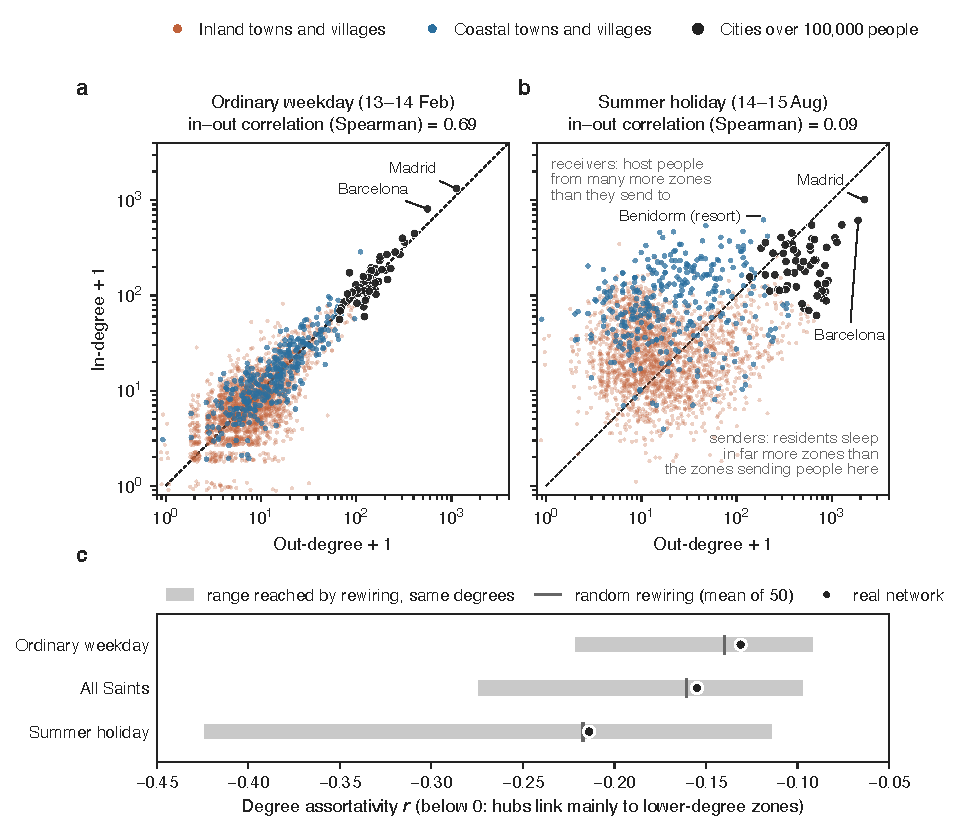
\includegraphics[width=\linewidth]{fig2_senders_receivers.pdf}
\caption{\textbf{On the summer night the network splits into senders and receivers.} On an ordinary night, zones that send people to many zones also receive people from many (points along the diagonal); on 14--15 August the cities move below the diagonal and coastal towns above it. \textbf{a, b}, Out-degree (zones its residents sleep in) against in-degree (zones whose residents sleep in it) of each zone on the ordinary night (a) and on 14--15 August (b), on logarithmic axes (degree $+1$, so that zones with degree zero can be shown); points are slightly jittered. \textbf{c}, Degree assortativity $r$ of the real network (dot), the mean of 50 degree-preserving rewirings (tick) and the range reached by maximally assortative and disassortative rewiring that keeps the network connected (bar; \citealp{zhou2007structural}).}
\label{fig:senders}
\end{figure}

The mixing of the network changes too. Degree assortativity falls from $-0.131$ on the ordinary night to $-0.214$ in summer: on holiday, the hubs link even more to zones of lower degree. But when I compared it with the null models, most of this turned out to come with the new degrees. Following \citet{zhou2007structural}, I rewire each network in three ways that keep every degree and a single connected component: towards the maximally assortative case, towards the maximally disassortative case, and at random (the maximal random case). The values reached by the first two move from $[-0.22,-0.09]$ to $[-0.42,-0.11]$, and the maximal random case gives $-0.140$ and $-0.217$, close to the real values (Figure~\ref{fig:senders}c); it reproduces 93\,\% of the real change from February. In other words, as in \citet{zhou2007structural}, the degree sequence constrains the mixing. A gap remains in August (about six standard deviations of the rewired networks), but it is small.

The rich club tells a similar story. The 50 best-connected zones, mostly cities, are linked in 80\,\% of their possible pairs on the ordinary night and 96\,\% in summer. Random networks with the same degrees give 66\,\% and 92\,\%, so the normalised rich-club coefficient, the ratio of the two, falls from 1.22 to 1.05 while the raw density rises. So on an ordinary night the cities form a club well beyond what their degrees produce; in summer, when they link to almost every zone, the degrees produce most of it, although the real club is still denser than the rewired ones. The bitmaps of the sorted adjacency matrix look alike on the three nights, the summer one denser (Figure~\ref{fig:bosam}).

Only one property goes clearly beyond the degrees and the rich club, and I did not expect it. Second-order mixing asks whether the neighbours of two linked zones are themselves alike. In summer it is $-0.289$, against $-0.252$ in rewired networks that keep the degrees and the rich-club curve $\phi(k)$, about 26 of their standard deviations lower; these networks also leave first-order mixing almost unchanged ($r=-0.217$ against $-0.214$), so the gap is not an effect of $r$; it remains with February's number of links (Table~\ref{tab:basic_full}). On the ordinary night it is close to zero ($0.000$ against $-0.023$), which is also above its null, by about 3.6 standard deviations, but in the opposite direction. In summer, if the other neighbours of one end of a link are well connected, those of the other end tend to be poorly connected, more than the degrees and the rich club require. The other summary, $R_{\max}$ (largest excess degree of the other neighbours), is above the same null on all three nights, so this summer departure is specific to $R_{\mathrm{avg}}$.

So the first answer is about structure: in summer the network turns into senders and receivers, its largest receivers are coastal, and most of its new mixing follows from the new degrees. It does not say who goes where.

\subsection{The roots pull every night, and in August the exodus generation pulls inland}\label{sec:res-roots}

On every night, ordinary or holiday, a city sends more of its residents to the provinces where more of them were born. Comparing two cities of the same province against the same destination, the pull of the roots, $\beta$ in equation~\eqref{eq:ppml}, is 0.53 on the ordinary night and 0.63 on 14--15 August, estimated on the 112 large cities that share a province with another one (Section~\ref{sec:method}). Put simply, a city with twice the share of residents born in a province sends about 1.45 times as many people there on a weekday in February, and 1.55 times in August. The pull is significant on every night tested ($p\le0.002$).

The same holds link by link. After removing what a gravity model of distance and size predicts, the correlation between the roots network and the overnight network, with cities permuted within their province (QAP), is 0.23 on the ordinary night and 0.48 on 14--15 August ($p<0.001$, 2,000 permutations); correlating the change in these residuals between the two nights with the roots gives $+0.10$ ($p<0.001$). Whether holidays make the pull stronger on average in the count regression is less clear, because it depends on which night I compare with. Against the February night the summer increase is $+0.096$ (95\,\% interval $-0.031$ to $0.242$, $p=0.18$); against October weekdays it is $+0.137$ ($0.048$ to $0.238$, $p=0.006$). On Christmas Eve the increase against February is $+0.065$ ($p=0.019$). But the average mixes groups that move in opposite directions, and splitting the census by group shows this (Figure~\ref{fig:roots}).

\begin{figure}[t]
\centering
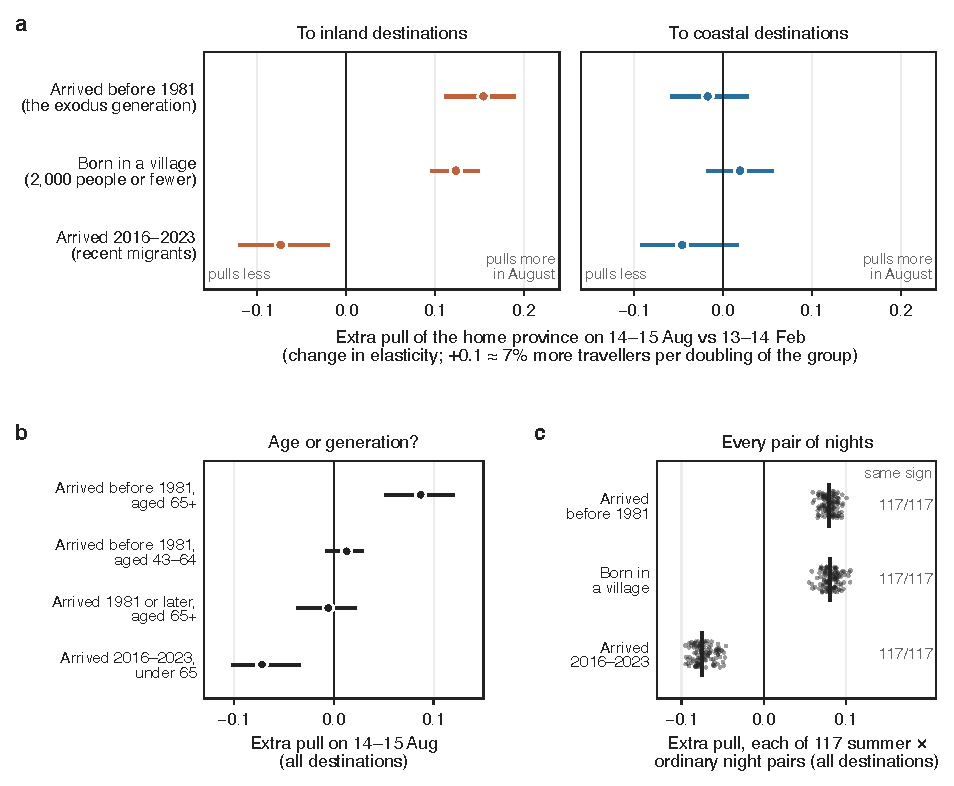
\includegraphics[width=\linewidth]{fig3_roots_generation.pdf}
\caption{\textbf{The extra summer pull of the province of birth comes from the exodus generation and goes inland.} Change in the pull of the roots ($\beta$ in equation~\ref{eq:ppml}) between 14--15 August and 13--14 February for each census group. Points right of zero: cities with a larger share of the group born in a province send relatively more people there in August than in February (shares describe residents; the outcome counts all stays from the city). Same 675 cities and 44 origin provinces for every estimate; bars are 95\,\% wild cluster bootstrap intervals; $+0.1$ means that the expected-flow multiplier for twice the group's share is about 7\,\% larger in August. \textbf{a}, Stays in inland and in coastal zones. \textbf{b}, Groups split by age. \textbf{c}, Each of the 117 pairs of one summer night and one February night.}
\label{fig:roots}
\end{figure}

Residents who arrived in their current province before 1981, most of them the generation of the exodus, pull harder in August: $+0.084$ (95\,\% interval 0.046 to 0.117, $p<0.001$). So do residents born in a village of 2,000 inhabitants or fewer: $+0.086$ (0.062 to 0.110). Residents who arrived in 2016--2023 pull less: $-0.072$ ($-0.114$ to $-0.020$). The extra pull is found inland. For stays in inland zones, the increase is $+0.154$ for the pre-1981 group (0.111 to 0.190) and $+0.123$ for the village-born (0.095 to 0.150); for stays on the coast it is $-0.017$ ($-0.059$ to $0.029$) and $+0.019$ ($-0.018$ to $0.056$), and no change can be detected against February (against October, the village-born coastal increase becomes significant).

These results could come from age, from unusual nights or from the baseline, so I checked all three. Age first: the exodus generation is old, and older people may simply travel differently. Splitting the groups by age, residents aged 65 or more who arrived in 1981 or later show no detectable extra pull ($-0.006$, interval $-0.038$ to $0.023$), while those aged 65 or more who arrived before 1981 show $+0.087$ ($0.051$ to $0.121$); pre-1981 arrivals aged 43--64 show a small increase that cannot be told from zero ($+0.013$). With the share of residents born in the province and aged 65 or more added to the model, the pre-1981 increase stays at $+0.060$ ($p<0.001$). Then the nights: for the pre-1981, village-born and recent groups, the sign is the same in all 117 pairs of a summer night and a February night, and the pre-1981 result stays between $+0.072$ and $+0.089$ when any one of the 44 provinces is left out. Finally the baseline: against the mean of October weekdays, the increases are $+0.086$ and $+0.093$. The recent-arrival result is less firm: against October it is $-0.032$ ($p=0.06$), and on the 2022 nights it cannot be detected (although the 2024 census groups include people who had not yet arrived in 2022).

Other holidays point the same way with smaller sizes: at Easter (the night ending on Good Friday) the pre-1981 group adds $+0.057$ and the village-born $+0.068$; on Christmas Eve, $+0.026$ and $+0.029$, and recent migrants no longer pull less.

\subsection{The emptied villages switch from senders to receivers}\label{sec:res-villages}

The villages that lost most people show the same pattern from the other side (Figure~\ref{fig:villages}). On an ordinary night, 24\,\% of the fifth of zones that lost most population receive more people than they send. On 14--15 August, 99\,\% do, and on Christmas Eve more than 99\,\%. Across all zones, the share of net receivers goes from 41\,\% to 65\,\% in August and 81\,\% at Christmas, while the large cities empty: Madrid's net balance, (in $-$ out)/(in $+$ out), goes from $+0.07$ to $-0.80$ in August.

\begin{figure}[t]
\centering
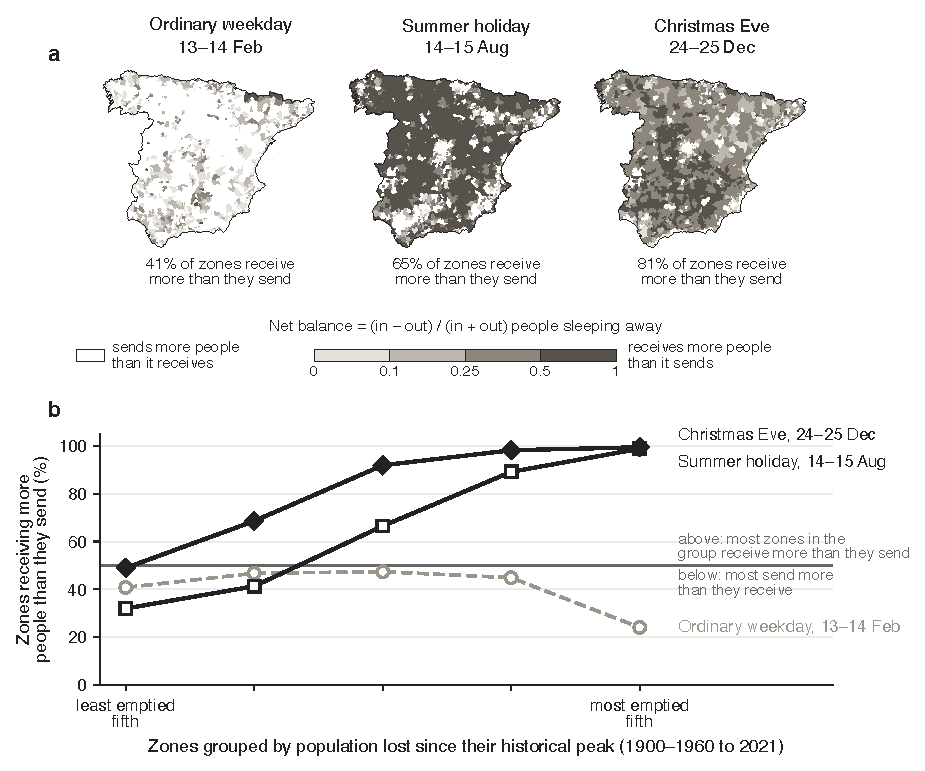
\includegraphics[width=0.93\linewidth]{fig4_villages.pdf}
\caption{\textbf{Emptied villages switch from sending people to receiving them.} \textbf{a}, Net balance, (in $-$ out)/(in $+$ out) of people sleeping away from home, of each of the 2,435 zones; white zones send more people than they receive. \textbf{b}, Share of zones that receive more than they send, by fifths of population lost since the 1900--1960 peak (2,376 zones with both overnight and population data). Greys distinguish nights.}
\label{fig:villages}
\end{figure}

The switch is still there after the controls. In the regression on the rank of loss, which holds fixed population, the number of municipalities in a zone, area, the coast, the distance to the nearest city and province, the chance of being a net receiver on 14--15 August is 39 percentage points higher for the most emptied zone than for the least emptied (95\,\% interval 23 to 55), and 44 points higher among zones made of a single municipality. On the ordinary night the difference goes the other way ($-12$ points, not significant). The summer result holds on all 9 sister nights and in 2022 and 2023.

The two holidays reach the same result in different ways. In August, the number of visitors (people from other zones sleeping there) to the most emptied zones is not detectably different from that of comparable zones that lost little population ($-0.05$ in logs, interval $-0.40$ to $0.30$); what differs is departures, with about half as many residents per head sleeping away. On Christmas Eve, the net gain per resident, (in $-$ out)/population, also rises against February. The stock of non-primary dwellings in the 2021 census \citep{ine2023viviendas}, which includes second homes, behaves differently on the two nights: adding its share of all dwellings to the regression of the August-to-February ratio of visitors on population loss reduces the coefficient of loss by 48\,\% in August (interval 22 to 82\,\%) and by 2\,\% on Christmas Eve. This is consistent with second homes mattering more in summer, but the data do not show where any visitor sleeps.

\subsection{All Saints: a family holiday away from the coast}\label{sec:res-allsaints}

All Saints is a family holiday when the coast pulls much less: inland towns and villages received twice as many people sleeping far from home as the coast (0.90 against 0.45 million; Figure~\ref{fig:calendar}). Its network keeps most of its reciprocity (0.48, against 0.24 in summer) and a rich club well above the rewired networks (0.91 against 0.81; Table~\ref{tab:basic}). The roots and the villages still point the same way as in summer, with smaller sizes: against February, the pre-1981 group adds $+0.038$ ($p=0.03$) and the village-born $+0.032$ ($p=0.01$), and 94\,\% of the most emptied fifth of zones receive more people than they send.

\subsection{What did not survive}\label{sec:res-failed}

Two results that looked good at first did not pass the checks. First, in raw means the coreness of emptied villages (the highest $k$-core a zone belongs to) rose sharply in summer, but among zones of similar size and location it falls behind by 9.4 shells, a fall that degree-preserving rewiring reproduces ($-8.9$). Second, the communities of the bipartite network of cities and destinations looked like scattered ``summer territories''; they beat a gravity null (weighted bipartite modularity, Leiden, 0.170 against 0.115 in August) but are more compact than it, not less (71\,\% of communities split into separate geographic pieces, against 99\,\%).
